\documentclass{standalone}
\usepackage{tikz}

\usetikzlibrary{matrix,positioning,shapes.arrows}

\tikzset{ 
table/.style={
  matrix of nodes,
  row sep=-\pgflinewidth,
  column sep=-\pgflinewidth,
  nodes={rectangle,draw,text width=1.25ex,align=center},
  text depth=0.25ex,
  text height=1ex,
  nodes in empty cells
  },
%texto/.style={font=\footnotesize\sffamily},
%title/.style={font=\small\sffamily}
}

\begin{document}
    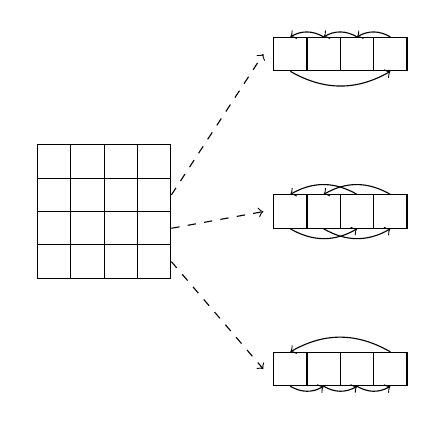
\begin{tikzpicture}
        \matrix [table] (m1)
        {
             & & & \\ 
             & & & \\
             & & & \\
             & & & \\
        };
        \matrix [table, right of=m1, node distance=3cm] (r2)
        {
            & & & \\
        };

        \matrix [table, above of=r2, node distance=2cm] (r1)
        {
            & & & \\
        };
        
        \matrix [table, below of=r2, node distance=2cm] (r3)
        {
            & & & \\
        };
        
        \draw[->] (r1-1-2.north) to [bend right] (r1-1-1.north);
        \draw[->] (r1-1-3.north) to [bend right] (r1-1-2.north);
        \draw[->] (r1-1-4.north) to [bend right] (r1-1-3.north);
        \draw[->] (r1-1-1.south) to [bend right] (r1-1-4.south);

        \draw[->] (r2-1-3.north) to [bend right] (r2-1-1.north);
        \draw[->] (r2-1-4.north) to [bend right] (r2-1-2.north);
        \draw[->] (r2-1-1.south) to [bend right] (r2-1-3.south);
        \draw[->] (r2-1-2.south) to [bend right] (r2-1-4.south);

        \draw[->] (r3-1-4.north) to [bend right] (r3-1-1.north);
        \draw[->] (r3-1-1.south) to [bend right] (r3-1-2.south);
        \draw[->] (r3-1-2.south) to [bend right] (r3-1-3.south);
        \draw[->] (r3-1-3.south) to [bend right] (r3-1-4.south);

        \draw[dashed, ->] (m1-2-4.east) -- (r1.west);
        \draw[dashed, ->] (m1-3-4.east) -- (r2.west);
        \draw[dashed, ->] (m1-4-4.east) -- (r3.west);
    \end{tikzpicture}
\end{document}